%-----------------------------------------------------------------------------------------------%
%
% Maret 2019
% Template Latex untuk Tugas Akhir Program Studi Sistem informasi ini
% dikembangkan oleh Inggih Permana (inggihjava@gmail.com)
%
% Template ini dikembangkan dari template yang dibuat oleh Andreas Febrian (Fasilkom UI 2003).
%
% Orang yang cerdas adalah orang yang paling banyak mengingat kematian.
%
%-----------------------------------------------------------------------------------------------%


%-----------------------------------------------------------------------------%
\chapter{\babTiga}
%-----------------------------------------------------------------------------%
Kerangka penelitian ini adalah langkah demi langkah dalam penyusunan Tugas Akhir mulai dari Tahap Perencanaan penelitian hingga Tahap Hasil dan Dokumentasi. Berikut ini adalah gambar Metodologi Penelitian dapat dilihat pada Gambar 3.1.
\begin{figure}
	\centering
	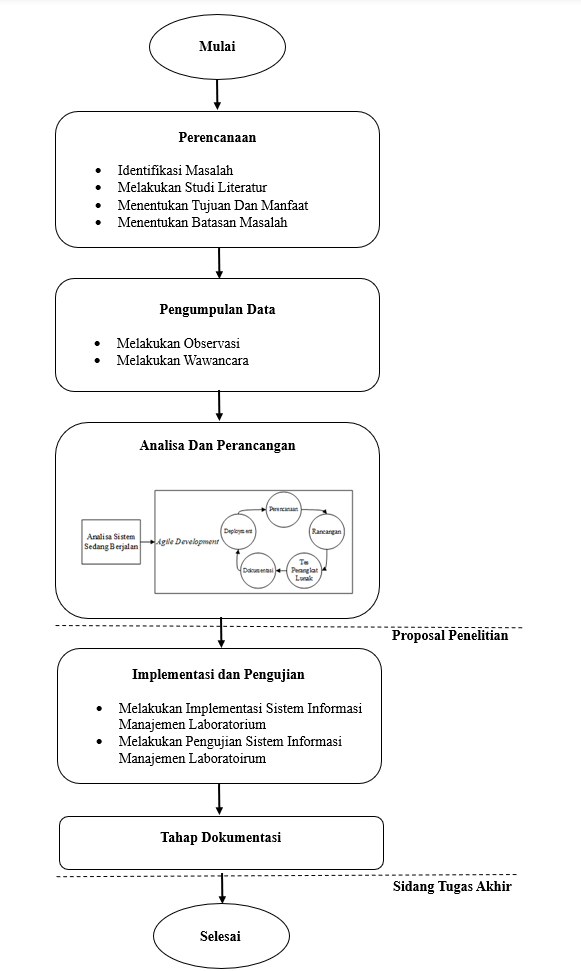
\includegraphics[width=0.82\linewidth]{konten//gambar/metodologi-penelitian.png}
	\caption{Metodologi Penelitian}
	\label{fig:enter-label}
\end{figure}
%-----------------------------------------------------------------------------%
\section{Tahap Perencanaan}
Langkah pertama dalam penelitian ini adalah mengidentifikasi masalah, studi literatur, menentukan tujuan dan manfaat, menentukan batasan masalah, menentukan data-data serta informasi yang dibutuhkan saat penelitian.

\subsection{Identifikasi Masalah}
Pada tahap ini, tujuan dari penelitian ini adalah untuk menemukan masalah dalam SITARIS SI untuk digunakan sebagai rumusan masalah. Dari masalah yang telah ditemukan dan disebutkan sebelumnya, rumusan masalah yang dihasilkan dari penelitian ini adalah “Bagaimana mengevaluasi kualitas SITARIS SI menggunakan metode ISO 9126 untuk dapat menentukan tingkat kualitas sistem dan kemudahan akses bagi pengguna serta memberikan rekomendasi untuk pengembangan sistem selanjutnya”.

\subsection{Studi Literatur}
Pada tahap ini, hal pertama yang dilakukan adalah melakukan penelitian literatur untuk mendapatkan informasi yang diperlukan untuk menulis tentang topik yang diangkat. Selain itu, kegiatan penelitian ini juga membantu mengetahui teori teori, serta metode dan teknik yang berkaitan dengan topik atau masalah yang akan digunakan untuk mencapai tujuan yang diinginkan. Teori yang digunakan di sini berasal dari artikel jurnal.

\subsection{Menentukan Tujuan dan Manfaat}
Pada tahap ini, akan dibahas tentang rumusan kalimat yang menunjukkan adanya hasil, tujuan penelitian, dan apa yang diperoleh setelah penelitian selesai.

\subsection{Menentukan Batasan Masalah}
Pada tahap ini, yang dilakukan adalah membatasi subjek penelitian. Untuk mengumpulkan masalah, penelitian ini menggunakan wawancardan dan kuisioner. Penelitian ini menggunakan metode Model ISO 9126 untuk menganalisis kualitas. Penelitian ini menggunakan teknik Probability Sampling, yaitu Proportionate Stratified Random Sampling, dan rumus slovin digunakan untuk menghitung jumlah sampel.

\section{Tahap Pengumpulan Data}
Pada tahap ini kegiatan yang dilakukan adalah menghimpun data baik data primer maupun data sekunder melalui kegiatan wawancara dan penyebaran kuesioner.

\subsection{Melakukan Wawancara}
Wawancara merupakan teknik pengumpulan data yang dilakukan melalui tatap muka dan tanya jawab langsung antara peneliti dan narasumber. Wawancara dilakukan untuk mendapatkan informasi secara tepat dan akurat dari narasumber yang terpercaya. Narasumber yang terkait pada penelitian ini yaitu bapak Tengku Khairil Ahsyar S.Kom., M.Kom., selaku Kepala Laboratorium Sistem Informasi.
\subsection{Menentukan Populasi dan Sampel}

\subsection{Membuat dan Menyebarkan Kuisioner}
Peneliti melakukan penyebaran kuisioner berdasarkan faktor atau karakteristik sesuai terkait evaluasi SITARIS SI ini. Setiap karakteristik memiliki sub karakteristik, masing– masing dari sub karakteristik yang nantinya akan disebarkan kepada responden. Responden yang terkait pada SITARIS SI adalah staff laboratorium dan mahasiswa UIN Suska Riau.
\section{Tahap Analisis dan Hasil}
\subsection{Menganalisis SITARIS SI}
\subsection{Menganalisis Pengolahan Kuisioner}
\subsection{Menganalisis Pengukuran Model ISO 9126}

\section{Tahap Kesimpulan dan Dokumentasi}
\subsection{Membuat persentase Kelayakan Sistem}
Persentase kelayakan website ini merupakan tahap proses untuk mengetahui persentase kelayakan dari sebuah website sehingga dapat ditarik kesimpulan apakah website tersebut termasuk kategori layak atau tidak website tersebut sehingga dapat ditarik kesimpulan apakah website tersebut dapat dikembangkan, dilanjutkan, atau diberhentikan. Besarnya persentase dapat dihitung dengan rumus berikut:

\[
\text{Persentase Kelayakan} = \frac{\text{Skor Aktual}(f)}{\text{Skor Ideal}} \times 100\%
\]

Dari rumus diatas diperoleh dengan cara menghitung skor
aktual (f) yang dibagi dengan skor ideal (n) kemudian dikalikan 100\%. Skor actual sendiri merupakan jumlah skor jawaban dari responden, sedangkan skor ideal (n) merupakan skor tertinggi jika responden tersebut memilih jawaban dengan skor tertinggi.

Selanjutnya persentase karakteristik tersebut akan dijumlah total untuk mendapatkan persentase keseluruhan. Rumus dalam menghitung persentase keseluruhan adalah sebagai berikut:

\[
\bar{x} = \frac{\sum x}{n}
\]

Keterangan :
X =Persentase rata-rata \\
x= Persentase total karakteristik
n =JumlahKarakteristik

Adapun tabel kelayakan menurut kelayakan menurut Arikunto (2008). Berikut tabelnya :

\begin{table}[h!]
	\centering
	\begin{tabular}{cc}
	\hline
	\textbf{Kategori}        & \textbf{Persentase} \\ \hline
	Sangat Baik              & 81\% - 100\%        \\
	Baik                     & 61\% - 80\%         \\
	Cukup Baik               & 41\% - 60\%         \\
	Tidak Baik               & 21\% - 40\%         \\
	Sangat Tidak Baik        & \textless 21\%      \\ \hline
	\end{tabular}
	\end{table}
	
	
\subsection{Membuat Rekomendasi dan Kesimpulan}
